\chapter{Parallel and distributed data processing}

Unlocking the potential of big data depends critically on parallel and \textbf{distributed processing (DP)}. Classical centralized methods become unsustainable and ineffective as data quantities grow exponentially. Big data workloads may be split up into smaller, more manageable jobs that can be carried out concurrently on many processing units by using \textbf{parallel processing (PP)}. Because of parallelism, huge speedups are possible and it is possible to handle enormous datasets in a reasonable amount of time. 

By distributing data and calculations over a cluster of computers, \textbf{DP} enhances parallelism. Both scalability and fault tolerance are provided by this configuration. To handle the increasing processing burden, more computers may be added to the cluster as the data volume rises. Because they duplicate data over many nodes, distributed file systems — like the \textbf{Hadoop Distributed File System (HDFS)} — ensure data availability and dependability.

By providing abstractions and \textbf{application programming interfaces (API)} that make it simpler to construct distributed systems, \textbf{Hadoop} and \textbf{Spark} have brought about a dramatic shift in the way that large data is handled. Using \textbf{MapReduce} functions, developers may specify calculations in \textbf{Hadoop} that are automatically parallelized and carried out on the cluster. By adding in memory processing capabilities and a large number of APIs for data manipulation, machine learning and graph processing, Spark expands on this idea.

\textbf{PP}, \textbf{DP} and \textbf{cloud infrastructure} working together have given big data analytics new opportunities. Elastic resources on cloud platforms may be dynamically provided and scaled according to the demands of the workload. Organizations may now handle and analyze enormous datasets without having to make large upfront infrastructure expenditures.

But in order to efficiently use \textbf{PP} and \textbf{DP} for big data for thorough analysis of resource management, task scheduling and data partitioning. The optimization of the allocation of tasks to available resources, the minimization of data transportation and the guaranteeing of load balance are all important functions that are performed by \textbf{scheduling algorithms}. Further sophisticated methods, like adaptive resource allocation and data locality-aware scheduling, may raise large \textbf{DP's} effectiveness and performance even further.

\section{Fundamentals of Parallel and Distributed Processing for Big Data}

Big data workloads have outgrown conventional sequential processing methods as data workloads have grown exponentially in recent years. A key \textbf{paradigm for effectively analyzing and obtaining value from enormous datasets is parallel and distributed processing}. "Why parallel and distributed processing is essential for big data" is the topic this part attempts to address.

Data sets involved in \textbf{big data} often surpass the storage and processing capacities of a single system by a significant margin, measuring in petabytes or exabytes. The scalability that is required to manage these enormous amounts of data may be achieved via the use of parallel and distributed architectures, which enable the data and computation to be dispersed among clusters of hundreds or thousands of commodity servers (\cite{Fadiya2018TheIO})\footnote[28]{\fullcite{Fadiya2018TheIO}}.

Distributed systems have the potential to significantly decrease processing times in comparison to sequential alternatives. This is achieved by \textbf{distributing data and tasks over a large number of nodes} that are capable of working in parallel. This offers significantly quicker insights and near-real-time analytics on large datasets. (\cite{Natesan2023ADF})\footnote[27]{\fullcite{Natesan2023ADF}}.

When compared to the use of costly supercomputers or specialist hardware, the utilization of distributed computing on commodity hardware clusters is much more \textbf{cost-effective} for the processing of large amounts of data (\cite{Fadiya2018TheIO})\footnotemark[28].

Large dataset processing over lengthy periods of time requires distributed frameworks to be able to \textbf{gracefully accept individual node failures} without impacting the overall workload (\cite{Wingerath2016RealtimeSP})\footnote[29]{\fullcite{Wingerath2016RealtimeSP}}. Few points sum up the principles of distributed and parallel computing.

\begin{itemize}
    \item Bigger datasets are \textbf{divided into smaller chunks} that may be handled concurrently and independently by many nodes. Typical methods include round-robin, hash and range partitioning;
    \item Often following patterns like \textbf{MapReduce, bulk synchronous parallel (BSP) }and \textbf{dataflow/stream processing}, algorithms are built to work on partitioned data in parallel.
    \item Specialized file systems, such as the \textbf{Hadoop Distributed File System (HDFS)}, provide a single view and enable data to be stored across a cluster.
    \item Resources (CPU, memory, etc.) are allocated to several simultaneous activities via \textbf{resource management }frameworks such as YARN;
    \item Parallel jobs require \textbf{coordination and synchronization} techniques, as does shared state across distributed nodes.
\end{itemize}

\section{Distributed Processing Frameworks for Big Data}

Among the first programming methods for distributed large data processing was \textbf{MapReduce}, made famous by Google. With the release of an open-source MapReduce implementation along with HDFS, Apache Hadoop emerged as the industry standard for batch processing large data (\cite{Fadiya2018TheIO})\footnote[28]{\fullcite{Fadiya2018TheIO}}.

\textbf{MapReduce and Hadoop} key characteristics are: Simple programming model with Map and Reduce phases; Automatic parallelization and distribution; Fault-tolerance through data replication and speculative execution; Scalability to thousands of nodes; However, MapReduce has limitations for iterative algorithms and real time processing. \textbf{Apache Spark}: in-memory processing for faster performance; Rich APIs in multiple languages; Support for batch, interactive and stream processing; Advanced analytics capabilities (machine learning, graph processing, etc.); Spark's Resilient Distributed Datasets (RDDs) provide fault-tolerant distributed memory abstraction. \textbf{Apache Storm}: Low-latency stream processing; At-least-once processing semantics; Native streaming (not micro-batch). \textbf{Apache Flink}: Both batch and stream processing; Exactly-once processing semantics; Lower latency than Spark Streaming. \textbf{Apache Samza}: Built for high-throughput event processing; Tightly integrated with Apache Kafka (\cite{Wingerath2016RealtimeSP})\footnotemark[29].

\section{Architectural Patterns for Big Data Processing}

The \textbf{Lambda Architecture}, proposed by Nathan Marz, combines batch and stream processing to balance latency, throughput and fault-tolerance . It consists of three layers:
\textbf{Batch Layer}: Periodically processes all historical data using a system like \textbf{Hadoop Speed Layer}: Processes real time data streams for low-latency views \textbf{Serving Laye}r: Responds to queries by merging batch and real time views This architecture provides comprehensive and accurate batch analytics along with approximate real time results (\cite{Wingerath2016RealtimeSP})\footnote[29]{\fullcite{Wingerath2016RealtimeSP}}.

\begin{figure}[H]
\caption{Lambda Architecture}
\centering
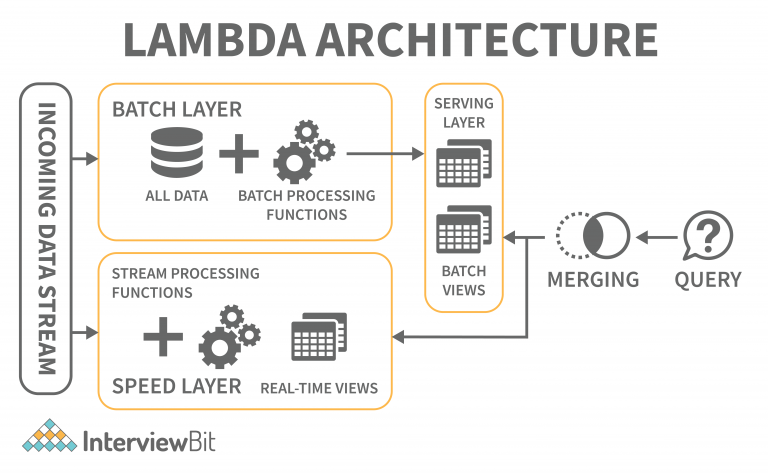
\includegraphics[width=1\linewidth]{images/Lambda-Architecture-768x475.png}
\small
\textit{Note.} The image depicts the Lambda architecture, a data processing framework designed for handling big data in real-time applications. \textbf{Batch Layer} — Processes all data and performs batch processing functions; \textbf{Speed Layer} — Handles stream processing and real-time views; \textbf{Serving Layer} — Provides batch views and merges data for queries; \textbf{Incoming Data Stream} — Feeds into both batch and speed layers; \textbf{Merging} — Combines batch and real-time processed data.
\textit{Creator.} (\cite{interviewBit})\footnote[39]{\fullcite{interviewBit}}
\end{figure}

The \textbf{Kappa Architecture}, introduced by Jay Kreps, simplifies the \textbf{Lambda Architecture} by treating both real time and historical data as streams. It uses a single stream processing engine capable of high-throughput reprocessing of historical data. \textbf{Key components}: Scalable message queue (e.g., Apache Kafka); Stream processor (e.g., Apache Samza); Serving database for processed results. This approach reduces complexity but requires a very robust stream processing system (\cite{Wingerath2016RealtimeSP})\footnote[29]{\fullcite{Wingerath2016RealtimeSP}}.

\begin{figure}[H]
\caption{Kappa Architecture}
\centering
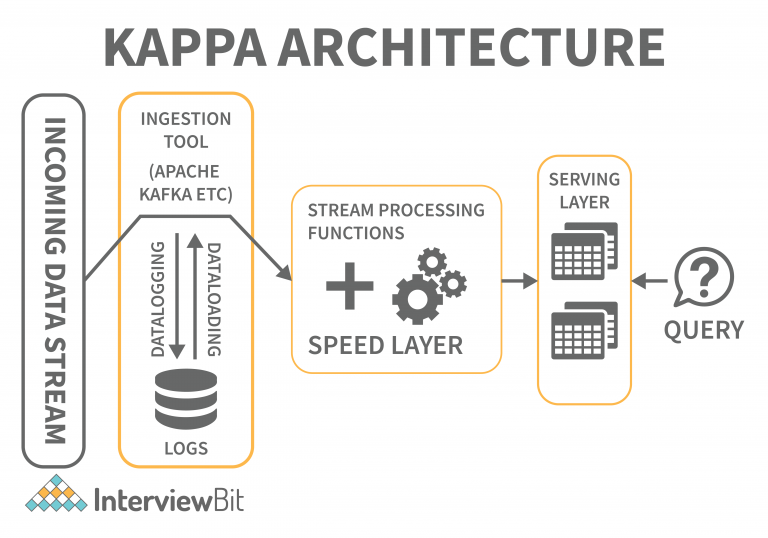
\includegraphics[width=1\linewidth]{images/Kappa-Architecture-768x538.png}
\small
\textit{Note.} The image depicts the Kappa Architecture, which is a data processing framework designed for handling real-time data streams. \textbf{Incoming Data Stream} — The starting point of the data flow; \textbf{Ingestion Tool} — Utilizes technologies like Apache Kafka for data intake; \textbf{Stream Processing Functions} — Core data processing layer; \textbf{Speed Layer} — Handles real-time data processing; \textbf{Serving Layer} — Presents processed data for querying; \textbf{Query Interface} — Allows users to interact with the processed data;
\textit{Creator.} (\cite{interviewBit})\footnote[39]{\fullcite{interviewBit}}
\end{figure}

\textbf{Microservices architectures} decompose big data applications into smaller, loosely-coupled services that can be developed, deployed and scaled independently. This approach can improve agility and scalability for complex big data systems (\cite{Wingerath2016RealtimeSP})\footnote[29]{\fullcite{Wingerath2016RealtimeSP}}, (\cite{interviewBit})\footnote[39]{\fullcite{interviewBit}}

\begin{figure}[H]
\caption{Microservice Architecture Style Structure}
\centering
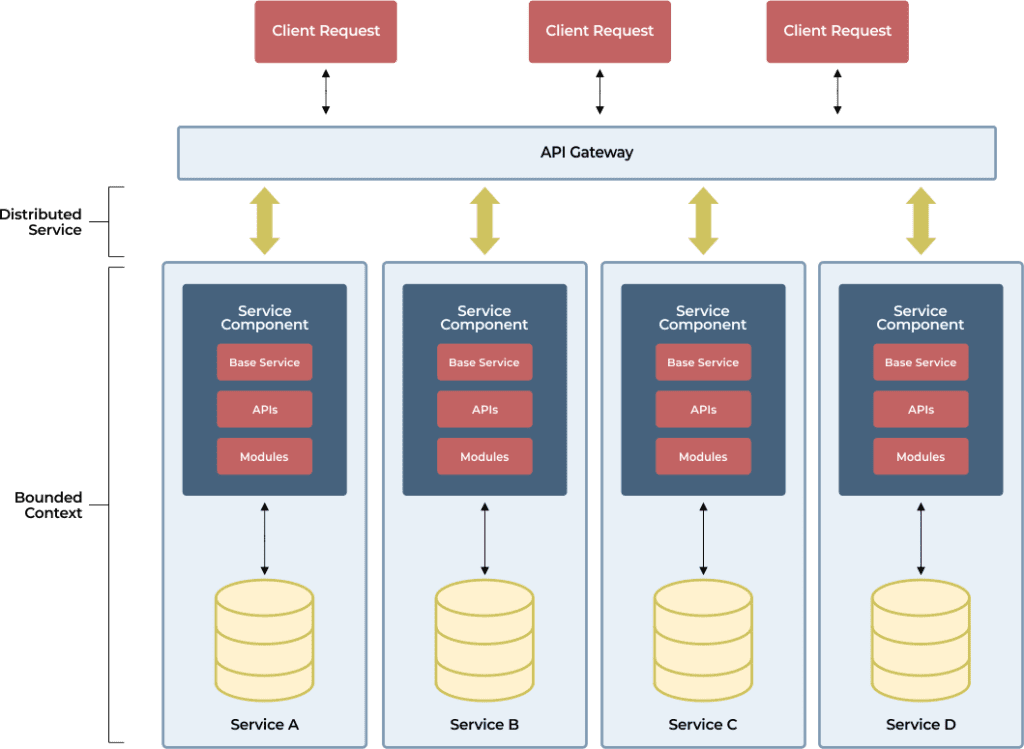
\includegraphics[width=1\linewidth]{images/Microservice-Architecture-img-1-1024x749.png}
\small
\textit{Note.} The image depicts a microservices architecture diagram. At the top of the diagram, there are three \textbf{"Client Request"} boxes, representing incoming requests from clients. Below the client requests is an \textbf{"API Gateway"} layer, which serves as the entry point for all client requests. The main body of the diagram shows \textbf{four separate services} (Service A, B, C, and D), representing a distributed service architecture.
\textit{Creator.} (\cite{micro})\footnote[40]{\fullcite{micro}}
\end{figure}

\section{Parallel Collections}

A tool developed to facilitate parallel programming and enhance multicore system performance is the \textbf{parallel collections} (\textbf{PC}) framework in Scala. Developers may take use of the potential of parallel computing without having to deal with low-level concurrency specifics thanks to this high-level abstraction for parallel data processing (\cite{parallel})\footnote[30]{\fullcite{parallel}}.

In Scala, \textbf{PCs} run by splitting up data into pieces and running many threads at once to process each chunk. Through the use of this divide-and-conquer strategy, it is possible to make effective use of the computer resources that are available. (\cite{parallel})\footnotemark[30].

\begin{table}[h!]
\caption{Parallel vs. sequential processing}
\begin{lstlisting}
val result = (1 to 1000000).filter(_ % 2 == 0).map(_ * 2).sum // Sequential processing
val parallelResult = (1 to 1000000).par.filter(_ % 2 == 0).map(_ * 2).sum // Parallel processing
\end{lstlisting}
\small
\textit{Note.} In this example, the parallel version (par) can potentially execute much faster on multi-core systems, especially for large datasets.
\textit{Creator.} Author's own work.
\end{table}

Scala's \textbf{PCs} framework provides parallel counterparts for most of the standard sequential collections including: \textbf{ParArray}, \textbf{ParVector}, \textbf{ParRange}, \textbf{ParSet} and \textbf{ParMap}. Each of these collections supports parallel operations while maintaining the semantics of their sequential counterparts (\cite{parallel})\footnotemark[30].

Though \textbf{PCs} may boost performance significantly, it is important to know when and how to utilize them. \textbf{They work well for}: Operations that benefit from parallelization more are those that need a lot of processing for each element; The overhead of parallelization is more justified for larger collections; Parallel processing works best for jobs when each component can be handled separately without interfering with others. \textbf{In terms of potential pitfalls}: Small collections may find that the costs of parallelization exceeds the advantages; Parallelization may not benefit I/O-intensive tasks; Due to the fact that some processes are non-associative, it is possible that when they are parallelized, they will generate different outcomes compared to their sequential counterparts (\cite{parallel})\footnote[30]{\fullcite{parallel}}.

\begin{table}[h!]
\caption{Non-associative operation}
\begin{lstlisting}
val numbers = (1 to 1000).toList
println(numbers.reduce(_ - _))        // Sequential - predictable result
println(numbers.par.reduce(_ - _))    // Parallel - potentially unpredictable result
\end{lstlisting}
\small
\textit{Note.} In this example, subtraction is non-associative, and the parallel version may produce different results in different runs.
\textit{Creator.} Author's own work.
\end{table}

\subsection{Task Support (TS)}
By use of the idea of \textbf{Task Support}, the Scala PCs framework enables \textbf{customization of task scheduling and execution}. Generally speaking, it is a part that offers fine-grained management of parallel operation execution. Customizing the execution environment for parallel operations is made possible by its function as an abstraction layer between the parallel collections and the underlying thread pool technology (\cite{task})\footnote[31]{\fullcite{task}}.

Scala's \textbf{PCs} by default employ a \textbf{ForkJoinTaskSupport} implementation that is derived from the Fork/Join framework seen in Java. For most general-purpose parallel processing requirements, this default solution works well. But Scala offers the ability to alter this behavior (\cite{task})\footnotemark[31].

\begin{table}[h!]
\caption{Non-associative operation}
\begin{lstlisting}
import scala.collection.parallel.TaskSupport
import scala.collection.parallel.ForkJoinTaskSupport
import java.util.concurrent.ForkJoinPool
val customParSeq = (1 to 10000).par
customParSeq.tasksupport = new ForkJoinTaskSupport(new ForkJoinPool(4))
\end{lstlisting}
\small
\textit{Note.} In this example, a custom \textbf{ForkJoinTaskSupport} is created with a specific \textbf{ForkJoinPool} that limits the parallelism to four threads. This level of control is particularly useful in scenarios where it is needed to manage system resources carefully or when working in environments with specific threading requirements.
\textit{Creator.} Author's own work.
\end{table}

\begin{itemize}
    \item \textbf{TS} decides how to divide, plan and control jobs among the available threads or processors;
    \item Depending on particular application requirements, it enables to choose or apply several task execution techniques;
    \item Through \textbf{TS}, the level of parallelism and resource utilization in their applications can be controlled (\cite{task})\footnote[31]{\fullcite{task}}.
\end{itemize}

\subsection{Performance Implications of Task Support}
\begin{itemize}
    \item Various \textbf{TS} implementations may modify the way work is distributed across threads, therefore affecting the ratio of parallelism overhead to efficient use of resources;
    \item Particularly for CPU-bound jobs, the frequency of context transitions may have an influence on overall performance depending on the thread pool design;
    \item \textbf{TS} setup done correctly guarantees best use of the system resources, avoiding CPU core oversubscription or underutilization (\cite{task})\footnotemark[31].
\end{itemize}

\begin{table}[h!]
\caption{Performance tuning with Task Support}
\begin{lstlisting}
import scala.collection.parallel.ForkJoinTaskSupport
import java.util.concurrent.ForkJoinPool
def parallelSum(numbers: Seq[Int], parallelism: Int): Int = {
  val par = numbers.par
  par.tasksupport = new ForkJoinTaskSupport(new ForkJoinPool(parallelism))
  par.sum}
val result = parallelSum((1 to 1000000), Runtime.getRuntime.availableProcessors())
\end{lstlisting}
\small
\textit{Note.} In this example, the parallelism is set to match the number of available processors, which can lead to more efficient execution on the given hardware 
\textit{Creator.} Author's own work.
\end{table}

When working with Task Support a few thing should be considered.
\begin{itemize}
    \item What is the application nature? CPU-bound vs. I/O-bound tasks may benefit from different \textbf{TS} configurations;
    \item To prevent overloading the level of parallelism has to be alligned with available resources;
    \item The size and complexity of the data being processed should determine TS strategy.
    \item Lastly, benchmarking. Different \textbf{TS} configurations should be tested to find the optimal setup for specific use case (\cite{task})\footnote[31]{\fullcite{task}}.
\end{itemize}

\section{Futures and Async Programming}

A \textbf{Future} represents a value that may not yet be available but will be at some point in the future. Handling asynchronous computations — like I/O operations or lengthy computations — without interrupting the primary execution thread depends on this notion. Non-blocking execution made possible by Futures also enables effective use of available resources. Finally, complicated asynchronous operations are made possible by the combination and transformation of many \textbf{Futures} (\cite{futures})\footnote[32]{\fullcite{futures}}.

\begin{table}[h!]
\caption{Futures}
\begin{lstlisting}
import scala.concurrent.Future
import scala.concurrent.ExecutionContext.Implicits.global
def fetchData(url: String): Future[String] = Future {
  Thread.sleep(1000) // Simulating a network call
  s"Data from $url"}
val dataFuture: Future[String] = fetchData("http://example.com/data")
\end{lstlisting}
\small
\textit{Note.} In this example, \textbf{fetchData} returns a \textbf{Future[String]}, allowing the program to continue execution while the data is being fetched asynchronously. 
\textit{Creator.} Author's own work.
\end{table}

Because Scala's \textbf{asnc/await} feature makes working with \textbf{Futures} more natural, asynchronous programming seems more sequential and reasonable. This helps especially with complicated jobs that need for coordination of many asynchronous actions. (\cite{futures})\footnotemark[32].

\begin{table}[h!]
\caption{Using Async/Await}
\begin{lstlisting}
import scala.concurrent.Future
import scala.concurrent.ExecutionContext.Implicits.global
import scala.async.Async.{async, await}
def processData(data: String): Future[Int] = Future {data.length} // Simulating data processing
val result: Future[Int] = async {val data = await(fetchData("http://example.com/data"))
  await(processData(data))}
\end{lstlisting}
\small
\textit{Note.} In this example, \textbf{async} creates a block that can contain await calls, which pause execution until the \textbf{Future} completes, without blocking the thread. This approach simplifies the handling of multiple dependent asynchronous operations.
\textit{Creator.} Author's own work.
\end{table}

\begin{table}[h!]
\caption{Error handling}
\begin{lstlisting}
def fallbackData: Future[String] = Future.successful("Fallback Data")
val robustDataFetch: Future[String] = fetchData("http://example.com/data")
  .recover { case _: Exception => "Default Data" }.fallbackTo(fallbackData)
\end{lstlisting}
\small
\textit{Note.} In this example, \textbf{recover} handles specific exceptions and provides a devault value, and \textbf{fallbackTo} tries an alternative \textbf{Future} if the firs one fails. This approach ensures that data pipelines can gracefully handle failures and continue processing with default or fallback data.
\textit{Creator.} Author's own work.
\end{table}

\begin{table}[h!]
\caption{Composition}
\begin{lstlisting}
def processMultipleDataSources(): Future[List[Int]] = {
  val dataSources = List("http://example.com/data1", "http://example.com/data2")
  Future.traverse(dataSources) { url =>
    for {
      data <- fetchData(url)
      result <- processData(data)
    } yield result}}
\end{lstlisting}
\small
\textit{Note.} This example demonstrates how multiple data sources can be processed in parallel. Futures can be composed to create complex workflows; Sequencing using \textbf{flatMap} or for-comprehensions or using \textbf{Future.traverse}.
\textit{Creator.} Author's own work.
\end{table}

\section{Akka Framework}

Akka is a toolkit and runtime for building highly concurrent, distributed and resilient message-driven applications on the JVM. It provides a higher level of abstraction for writing concurrent and distributed systems.

\subsection{Actor Model}

Programming idea and tool the \textbf{Akka Actor Model} was developed to make concurrent and distributed system development easier. For creating \textbf{parallel, distributed and failure-resistant applications}, it provides a higher degree of abstraction. Handling systems with components interacting in real time is particularly beneficial using this method, as in large-scale data processing jobs, Internet of Things applications, or responsive web services (\cite{kuhnReactiveDesignPatterns2017})\footnote[33]{\fullcite{kuhnReactiveDesignPatterns2017}}.

Fundamentally, the \textbf{Actor Model} centers on the notion of \textbf{"actors"} as the building blocks of computing. \textbf{Lightweight and self-contained, an actor captures state and behavior}. Actors interact only via message passing, which promotes component flexibility and aids in concurrent system complexity control (\cite{kuhnReactiveDesignPatterns2017})\footnotemark[33].

In the Akka implementation of the Actor Model, each actor possesses characteristics;

\begin{enumerate}
    \item An actor has its own private state that cannot be directly accessed or altered by other actors. This encapsulation aids in preventing concurrency issues such, as race conditions;
    \item Actors process messages one at a time, in a single-threaded manner within the actor. This characteristic eliminates the need for complex locking mechanisms within an actor's logic;
    \item When an actor receives a message it can change its state, communicate with actors, spawn new actors or decide how to process the next message;
    \item Actors, in the system, are designed to work whether they are situated locally (within the JVM) or remotely (on a different machine within the network).
\end{enumerate}

An important advantage of the \textbf{Actor Model} is its approach to handling errors. In Akka actors are structured in a hierarchy known as a \textbf{"supervisor hierarchy"}. If an actor encounters an error (such as throwing an exception) its supervisor. The actor that created it. Determines how to address the issue. This response could involve restarting the actor, halting its operation or escalating the problem to a higher level supervisor. This hierarchical supervision system enables management of failures. Facilitates graceful recovery from them (\cite{kuhnReactiveDesignPatterns2017})\footnotemark[33].

Leveraging the Actor Model also provides a means of application scalability. Distribution of actors among computers in a cluster is quite simple since actors communicate via messages. Clustering capabilities included into Akka allow actors to be dispersed across network nodes while addressing distributed computing issues such network communication and failure management (\cite{kuhnReactiveDesignPatterns2017})\footnotemark[33].

A well-known characteristic of the Akka Actor Model is its ability to support reactive programming ideas. Akka actors are designed to stay responsive, under loads recover from failures, scale based on demand and rely on asynchronous message passing for communication. With its characteristics, Akka is an excellent option for creating reactive systems that can manage concurrency and remain responsive under changing loads (\cite{kuhnReactiveDesignPatterns2017})\footnotemark[33].

When building data processing pipelines in the area of data engineering, the Akka Actor Model shows useful. Actors are components of a data pipeline that stand for certain processing or transformation operations. These pipeline stages are composed more simply with the message passing technique, and the fault tolerance features that are incorporated improve the reliability of data processing processes (\cite{kuhnReactiveDesignPatterns2017})\footnotemark[33].

As an example, some actors may be responsible for gathering data from various sources, while others would handle cleaning and transforming the data. Still others would be tasked with aggregating and evaluating the findings. For better performance, the actor model allows these procedures to be distributed over a machine cluster and parallelized (\cite{kuhnReactiveDesignPatterns2017})\footnote[33]{\fullcite{kuhnReactiveDesignPatterns2017}}.

\begin{table}[H]
\caption{Basic Actor Structure in Akka}
\begin{lstlisting}
import akka.actor.{Actor, ActorSystem, Props}
class DataProcessorActor extends Actor {var processedCount = 0
  def receive: Receive = {case data: String =>
      processedCount += 1
      println(s"Processing: $data (Total processed: $processedCount)")
    case "getCount" => sender() ! processedCount
    case _          => println("Unknown message")}}
val system = ActorSystem("DataEngineeringSystem")
val dataProcessor = system.actorOf(Props[DataProcessorActor], "dataProcessor")
dataProcessor ! "Sample data"
dataProcessor ! "getCount"
\end{lstlisting}
\small
\textit{Note.} In this example, \textbf{DataProcessorActor} encapsulates its state (\textbf{processedCount}) and defines its behavior in the \textbf{receive} method. It can process data and respond to queries about its internal state, all through message passing .
\textit{Creator.} Author's own work.
\end{table}

\begin{table}[H]
\caption{Actor Hierarchies and Supervision}
\begin{lstlisting}
class SupervisorActor extends Actor {
  val child1 = context.actorOf(Props[ChildActor], "child1")
  val child2 = context.actorOf(Props[ChildActor], "child2")
  def receive: Receive = { case msg => child1 ! msg // Forward message to child1}
  override val supervisorStrategy = OneForOneStrategy() {
      case _: ArithmeticException => Restart
      case _: Exception           => Stop}}
\end{lstlisting}
\small
\textit{Note.} In this example, Akka implements a hierarchical structure for actors, known as the \textbf{actor hierarchy}. Hierarchy allows for structured error handling and fault tolerance. The supervisor can decide how to handle failures in its child actors, such as restarting them or stopping them .
\textit{Creator.} Author's own work.
\end{table}

\subsection{Actors Advantage in Data Engineering}

\begin{table}[H]
\caption{Actors Scalability and Performance}
\begin{lstlisting}
val system = ActorSystem("DataProcessingSystem")
val router = system.actorOf(
  RoundRobinPool(10).props(Props[DataProcessorActor]),
  "dataProcessorRouter")
(1 to 1000).foreach { i =>
  router ! s"Data chunk $i"}
\end{lstlisting}
\small
\textit{Note.} This example creates a router with 10 instances of \textbf{DataProcessorActor}, distributing the workload across multiple actors for parallel processing. Actors are lightweight and can be created in large numbers, allowing for fine-grained parallelism in data processing tasks.
\textit{Creator.} Author's own work.
\end{table}

\begin{table}[H]
\caption{Actors Scalability and Performance}
\begin{lstlisting}
class AggregatorActor extends Actor {
  var sum = 0
  var count = 0
  def receive: Receive = {
    case value: Int =>
      sum += value
      count += 1
    case "getAverage" =>
      sender() ! (if (count > 0) sum.toDouble / count else 0)}}
\end{lstlisting}
\small
\textit{Note.} In this example, actor maintains a \textbf{running average}, demonstrating how stateful computations can be encapsulated within an actor. Actors can maintain state between messages, useful for stateful data processing operations.
\textit{Creator.} Author's own work.
\end{table}

\subsection{Reactive Streams}

\begin{figure}[H]
\caption{Reactive Streams}
\centering
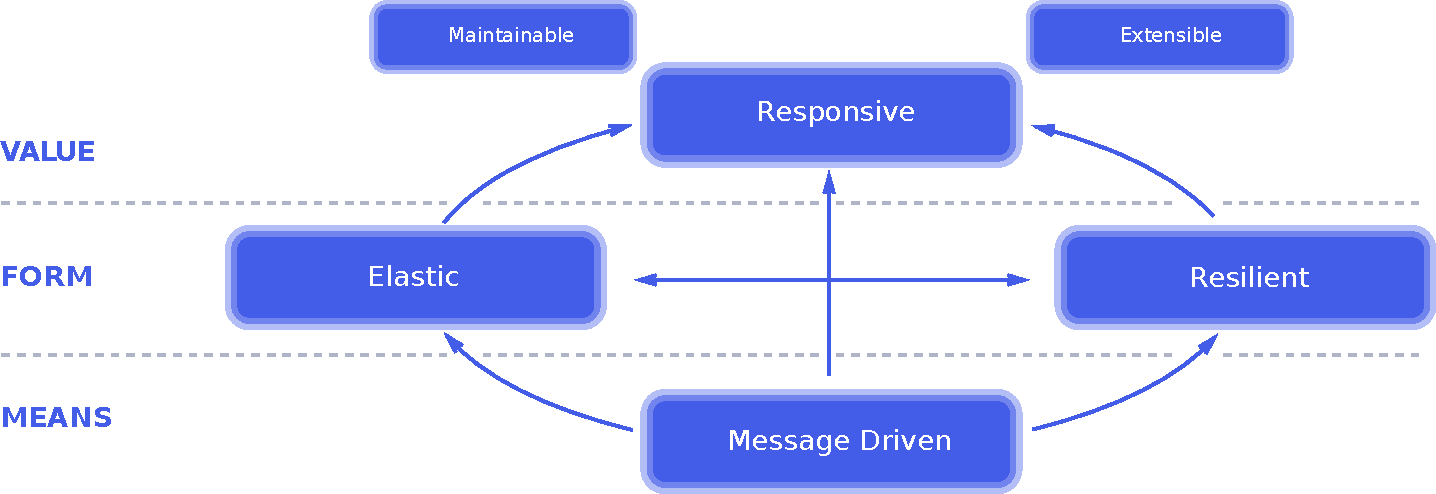
\includegraphics[width=1\linewidth]{images/reactive-traits.pdf}
\small
\textit{Note.} This diagram illustrates the key principles of Reactive Systems as outlined in the \textbf{Reactive Manifesto}. The diagram is divided into three layers: Value, Form, and Means. It showcases six core concepts of Reactive Systems. The layout emphasizes how these concepts interact and support each other.
\textit{Creator.} (\cite{stream})\footnote[34]{\fullcite{stream}}
\end{figure}

Standard Reactive Streams handle asynchronous stream processing under non-blocking demand. Within the field of distributed and parallel data processing, this technology provides a means of handling enormous amounts of data across several computers. It shows to be useful in data engineering situations where processing pipelines have to control throughput real-time data streams while maintaining system stability and responsiveness (\cite{kuhnReactiveDesignPatterns2017})\footnote[33]{\fullcite{kuhnReactiveDesignPatterns2017}}.

At its essence, Reactive Streams establishes a framework of interfaces and rules for facilitating asynchronous stream processing among components within a distributed system. The standard outlines four interfaces; Publisher, Subscriber, Subscription and Processor. These interfaces collaborate to facilitate the flow of data throughout a processing pipeline while effectively managing back pressure to sustain system stability amidst varying workloads (\cite{kuhnReactiveDesignPatterns2017})\footnotemark[33].

Reactive Streams offers various benefits in the field of distributed and parallel data processing; It enables non-blocking asynchronous data processing—a critical feature in distributed systems where components may process data at different speeds. Through asynchronous processing, quicker components are able to function without being delayed by slower ones, which maximizes the efficiency of the system (\cite{kuhnReactiveDesignPatterns2017})\footnotemark[33].

Its integrated system to manage back pressure is one of its main advantages. Different phases of a distributed data processing pipeline may be able to handle jobs to differing degrees. Back pressure is the ability of components to tell upstream components about their processing capabilities, therefore preventing quicker data producers from overpowering slower data users. This contributes to memory-related problems in distributed environments being avoided and system stability being maintained.
 (\cite{kuhnReactiveDesignPatterns2017})\footnotemark[33].

Reactive Streams supports constructing data processing pipelines modularly. Following the Reactive Streams interfaces, each step of the pipeline may be constructed as reusable components. This allows for more flexibility. Because of its modularity, which is in line with the ideas of functional programming, complex distributed data flows may be created using simple, clearly defined building components (\cite{kuhnReactiveDesignPatterns2017})\footnotemark[33].

Because Reactive Streams are asynchronous and can control back pressure, they are perfect for building scalable distributed data processing systems. More processing nodes may be added into the system as the amount of data grows, and Reactive Streams manages the data flow between them (\cite{kuhnReactiveDesignPatterns2017})\footnotemark[33].

While not included in the Reactive Streams definition directly, implementations often provide capabilities to manage failures in distributed settings. A known implementation of Reactive Streams, Akka Streams, for example, provides features for error handling and recovery in distributed stream processing situations (\cite{kuhnReactiveDesignPatterns2017})\footnotemark[33].

Reactive streams may be used in reality for many different facets of distributed and parallel data processing; building scalable, robust data ingestion pipelines that can handle large volumes of real-time data streams from many sources is one such uses (\cite{kuhnReactiveDesignPatterns2017})\footnote[33]{\fullcite{kuhnReactiveDesignPatterns2017}}.

Use of a back pressure mechanism prevents the ingestion process from overpowering subsequent processing phases. Reactive Streams processors, each specialized to a certain transformation aspect, may be used to break down complex data transformation algorithms. Parallel processing is made possible by the dispersal of these processors across nodes. Reactive Streams may be effectively used by real time analytics pipelines to process and analyze data as it moves through the system. Analytical jobs are made easier to complete by Reactive Streams' asynchronous design. Reactive Streams help to control the data flow while exporting processed data to systems so as to avoid overwhelming the receiving systems (\cite{kuhnReactiveDesignPatterns2017})\footnotemark[33].

Reactive Streams standard is followed by many libraries and frameworks in the Scala ecosystem, which makes it easier to include these ideas into data engineering projects. As one example, Akka Streams provides a high-level DSL for building Reactive Streams compliant stream processing pipelines. With its smooth integration with the Akkas actor paradigm, distributed and reactive data processing systems may be built (\cite{kuhnReactiveDesignPatterns2017})\footnote[33]{\fullcite{kuhnReactiveDesignPatterns2017}}.

\begin{table}[H]
\caption{Asynchronous Processing}
\begin{lstlisting}
import akka.stream.scaladsl._
import scala.concurrent.Future
def processData(data: String): Future[String] = Future {
  // Simulating asynchronous processing
  Thread.sleep(100)
  data.toUpperCase}
val source: Source[String, NotUsed] = Source(List("data1", "data2", "data3"))
val flow: Flow[String, String, NotUsed] = Flow[String].mapAsync(4)(processData)
val sink: Sink[String, Future[Done]] = Sink.foreach(println)
source.via(flow).runWith(sink)
\end{lstlisting}
\small
\textit{Note.} In this example, \textbf{mapAsync} allows for asynchronous processing of each element in the stream, maintaining responsiveness even with time-consuming operations. \textbf{Reactive Streams} are designed to \textbf{handle data asynchronously}, allowing for non-blocking operations. This is crucial for building responsive systems that can handle high volumes of data without becoming unresponsive.
\textit{Creator.} Author's own work.
\end{table}

\begin{table}[H]
\caption{Non-blocking Back Pressure}
\begin{lstlisting}
import akka.stream.OverflowStrategy
val bufferingFlow: Flow[Int, Int, NotUsed] = Flow[Int]
  .buffer(10, OverflowStrategy.backpressure)
  .map { x =>
    Thread.sleep(100) // Simulate slow processing
    x * 2}
Source(1 to 100)
  .via(bufferingFlow)
  .runWith(Sink.foreach(println)))
\end{lstlisting}
\small
\textit{Note.} In this example, the buffer stage with OverflowStrategy.backpressure ensures that if the downstream processing is slow, the upstream will be notified to slow down its production rate. \textbf{Back pressure} is a mechanism that allows consumers to signal to producers about their current capacity to handle data. This prevents fast producers from overwhelming slow consumers, ensuring system stability.
\textit{Creator.} Author's own work.
\end{table}

\begin{table}[H]
\caption{Stream Composability}
\begin{lstlisting}
def filterEven: Flow[Int, Int, NotUsed] = Flow[Int].filter(_ % 2 == 0)
def multiply(factor: Int): Flow[Int, Int, NotUsed] = Flow[Int].map(_ * factor)
def logElement: Flow[Int, Int, NotUsed] = Flow[Int].map { x => println(s"Processing: $x") x}
val composedFlow: Flow[Int, Int, NotUsed] = filterEven.via(multiply(2)).via(logElement)
Source(1 to 10).via(composedFlow).runWith(Sink.foreach(println))
\end{lstlisting}
\small
\textit{Note.} This example demonstrates how multiple simple flows can be composed to create a more complex data processing pipeline. \textbf{Reactive Streams} are designed to be composable, allowing complex data processing pipelines to be built from simpler, reusable components.
\textit{Creator.} Author's own work.
\end{table}

\begin{table}[H]
\caption{Bounded Resource Consumption}
\begin{lstlisting}
import akka.stream.ThrottleMode
val throttledSource: Source[Int, NotUsed] = Source(1 to 100).throttle(10, 1.second, 5, ThrottleMode.shaping)
throttledSource.runWith(Sink.foreach(println))
\end{lstlisting}
\small
\textit{Note.} This example uses throttling to limit the rate of data flow, ensuring bounded resource consumption even with fast producers. \textbf{Reactive Streams} ensure that system resources are used efficiently by \textbf{bounding} the number of elements that can be in-flight at any given time. This prevents memory overflow and system crashes due to unbounded queues.
\textit{Creator.} Author's own work.
\end{table}

\begin{table}[H]
\caption{Bounded Resource Consumption}
\begin{lstlisting}
import akka.stream.scaladsl._
import akka.{Done, NotUsed}
import scala.concurrent.Future
case class SensorData(id: String, value: Double)
val sensorSource: Source[SensorData, NotUsed] = Source.repeat(0).map { i =>
  SensorData(s"sensor-${i % 10}", math.random())
}.throttle(100, 1.second)
val aggregationFlow: Flow[SensorData, (String, Double), NotUsed] = 
  Flow[SensorData]
    .groupBy(10, _.id)
    .fold((0.0, 0)) { case ((sum, count), data) => (sum + data.value, count + 1) }
    .map { case (id, (sum, count)) => (id, sum / count) }
    .mergeSubstreams
val persistSink: Sink[(String, Double), Future[Done]] = 
  Sink.foreach { case (id, avg) => println(s"Sensor $id average: $avg") }
sensorSource
  .via(aggregationFlow)
  .runWith(persistSink)
\end{lstlisting}
\small
\textit{Note.} This example demonstrates a more complex data engineering scenario using Reactive Streams principles in Scala. It simulates sensor data processing, including throttling, grouping, aggregation, and persistence.
\textit{Creator.} Author's own work.
\end{table}

\section{Apache Spark}

Scalable and robust distributed computing was the driving force for the creation of the \textbf{Apache Sparks} framework. Spark works essentially with a master worker configuration, in which a cluster of executor nodes is divided up into work by a \textbf{central coordinator (called the driver software)}. Using the combined computing power of several computers, this method enables Spark to manage datasets efficiently (\cite{Kona2023LeveragingSA})\footnote[16]{\fullcite{Kona2023LeveragingSA}}.


\textbf{Spark} applications containing the function and taking on the duty of initializing the \textbf{SparkContext}, which functions as a gateway to all of Spark's capabilities, begins with the \textbf{driver program}. For resource and task scheduling throughout the cluster, the \textbf{SparkContext} works with cluster managers such as \textbf{YARN}, \textbf{Mesos}, or \textbf{Spark's standalone cluster manager}. Spark runs well on cluster managers thanks to this degree of abstraction; application code is not needed to be changed (\cite{Kona2023LeveragingSA})\footnotemark[16].

Operation of a Spark cluster involves \textbf{executor nodes}. Every executor runs on a worker node and is a Java Virtual Machine (JVM) process. The driver software assigns tasks to these executors, which also have to handle data storage in memory or on disk. Caching data in memory is what sets Spark apart from disk-based systems and improves algorithm and interactive data analysis performance (\cite{Kona2023LeveragingSA})\footnotemark[16].


\textbf{Resilient Distributed Datasets (RDDs)} are the foundation of \textbf{Spark's execution model}. \textbf{RDDs} are collections of records that are immutable, partitioned and can be operated on in parallel. They are the foundation of Spark's technique for fault tolerance. If a node fails and a portion of an RDD disappears, Spark may rebuild it using data about its past kept in the RDD. This approach spares Spark from costly data duplication and allows it to recover from errors (\cite{Kona2023LeveragingSA})\footnotemark[16]. 

A \textbf{Directed Acyclic Graph (DAG) scheduler} is used by the Spark engine to improve the execution of complicated processes. When an operation is performed on an RDD, Spark inspects its history of actions. Forms an execution plan. Substages of this plan are then made up of jobs that may execute simultaneously across the cluster. The DAG scheduler excels at optimizing operations flow and reducing data movement over the network, which significantly boosts Spark's performance edge (\cite{Kona2023LeveragingSA})\footnotemark[16]. 

\textbf{Spark} integrates libraries that enhance its capabilities beyond basic tasks, in addition to the essential components that make up the Spark framework. For structured data processing, \textbf{Spark SQL}; for real-time data streams, \textbf{Spark Streaming}; for machine learning tasks, \textbf{MLlib}; and for graph computations, \textbf{GraphX}. Because these libraries interface directly with the main engine, developers may combine many data processing techniques into a single application. A memory management system included into Sparks design additionally cleverly decides how to allocate memory for computational and data storage activities (\cite{Kona2023LeveragingSA})\footnotemark[16].

By use of this approach, known as \textbf{Unified Memory Management}, Spark may modify the memory allocation for execution and caching according to the workload. Sparks performance in managing workloads ranging from batch processing to interactive queries is partly attributed to this adaptive memory management (\cite{Kona2023LeveragingSA})\footnotemark[16].

Spark's modular architecture also translates to its data source and format adaptability. Among the many data sources Spark can read from and write to are cloud storage systems, conventional relational databases and distributed file systems like HDFS. This adaptability makes Spark possible to be integrated into current data contexts, makes complex data processing pipelines that straddle many storage systems and data types possible (\cite{Kona2023LeveragingSA})\footnote[16]{\fullcite{Kona2023LeveragingSA}}.

\subsection{Spark DataFrames and APIs}

With its higher-level abstraction approach than the fundamental Resilient Distributed Datasets (RDDs), Spark \textbf{DataFrames} and \textbf{Datasets APIs} represent a breakthrough in Spark data processing capabilities. Using structured and semi-structured data should be made easy for users with the help of these APIs. They combine working with local data sets with the strength of Spark distributed computation (\cite{Chambers2018SparkTD})\footnote[35]{\fullcite{Chambers2018SparkTD}}.

Introduced in Spark 1.3 \textbf{DataFrames} provide a distributed collection of data structured into named columns. Essentially, they are \textbf{equivalent to tables in a database or data frames in R/Python}. Enhanced by Spark distributed computing prowess. DataFrames are tailored for handling of large-scale structured data. They come with a domain-specific language (\textbf{DSL}) for manipulating distributed data allowing operations, like filtering, grouping and aggregation to be expressed naturally and concisely compared to RDDs (\cite{Chambers2018SparkTD})\footnotemark[35].

Using optimization techniques to produce effective query plans, Spark SQL's Catalyst optimizer is used by the \textbf{DataFrame API}. Behind-the-scenes optimization allows developers to concentrate on communicating their data modifications while Spark manages the effective cluster-wide execution. Predicate pushdown, column trimming and reordering joins are just a few of the improvements the Catalyst optimizer can undertake to significantly improve query speed in data processing processes (\cite{Chambers2018SparkTD})\footnotemark[35].

Introduced with Spark 1.6, \textbf{datasets} extend the DataFrame notion by providing a strongly-typed API that combines the benefits of RDDs type safety with the DataFrame API's efficiency. Because datasets make advantage of Scala compile-time type safety, they are especially well-suited for usage with Scala. This feature produces dependable code by allowing problems to be found at compile time that would only be detected at runtime with DataFrames (\cite{Chambers2018SparkTD})\footnotemark[35].

A DataFrame in Scala is just an untyped JVM object represented by Row in a type alias for Dataset[Row]. Scala's DataFrames and Datasets integration facilitates a switch between typed and untyped APIs, letting developers choose the degree of type safety that most closely fits their needs. Compile time type safety and the Catalyst optimizer's improvements may be benefited by developers working with datasets that include case classes (\cite{Chambers2018SparkTD})\footnotemark[35].

DataFrames and Datasets have the same crucial feature of being able to automatically infer schemas from data sources. Working with data sources is made easier by the inferred schemas and Spark SQL's support for reading data formats such JSON, Parquet and Avro. When automated schema inference fails, developers may manually construct schemas using both APIs to have control over column names and data types (\cite{Chambers2018SparkTD})\footnotemark[35].

The DataFrames and Datasets APIs also provide a variety of data manipulation and analysis capabilities. Along with more sophisticated chores like window functions and intricate type manipulations, these operations encompass filtering, sorting and aggregating data. Many of these procedures are stated in easily understandable domain-specific languages (DSLs). This opens up complicated data transformations to developers without distributed computing experience (\cite{Chambers2018SparkTD})\footnotemark[35].

Moreover, interoperability of the DataFrames and Datasets APIs with Spark components is one of their main benefits. Building machine learning pipelines may be streamlined, for instance, by the smooth interaction of machine learning algorithms in Spark MLlib with DataFrames. In a similar vein, batch and stream processing may be integrated inside of a single application using Spark Streaming's ability to generate and consume data frames (\cite{Chambers2018SparkTD})\footnotemark[35].


When managing data processing chores, DataFrames and Datasets often perform better than RDDs. Their power to use the improved execution engine of Spark SQL, which includes rule- and cost-based improvements, is what makes them successful. Datasets' encoders also allow JVM objects to be serialized and deserialized, which lowers memory use and improves speed when managing complex data formats (\cite{Chambers2018SparkTD})\footnote[35]{\fullcite{Chambers2018SparkTD}}.